\section{Keys} \label{sec:spec:keys}

\subsection{Public Parameters}

Public keys use some public parameters that are shared by many key
pairs:
\begin{enumerate}
\item The cyclotomic polynomial $\phi = x^n+1$, where $n = 2^\kappa$ is a power of $2$. We note that $\phi$ is monic and irreducible.
\item A modulus $q \in \bN^\star$. In \falcon, $q = 12289$. We note that $(\phi \bmod q)$ splits over $\bZ_q[x]$.
\item A real bound $\sqsignorm > 0$.
\item Standard deviations $\sigma$ and $\sigmin < \sigmax$.
\item A signature bytelength \sigbytelen.
\end{enumerate}
%  Many of our algorithms are different whether we take $\phi = x^n+1$ or $\phi = x^n - x^{n/2} + 1$. Since $x^n+1$ is a binary polynomial and its working with it implies manipulating binary trees, we will often refer to situations involving it as \emph{binary cases}; similarly, since $x^n - x^{n/2} + 1$ is a ternary polynomial and implies ternary trees, situations involving it will be called \emph{ternary cases}. In \falcon, we do not consider values of $n$ higher than $1024$.
 
For clarity, public parameters may be omitted (\eg in algorithms' headers) when clear from context.

% The definition can be extended to larger primes $q$, and degrees $n$
% larger than $1024$. Some operations are made more efficient by choosing
% $q$ such that $q$ is prime and $q = 1 \bmod 2n$; for $n\leq 1024$, $q =
% 18433$ is such an alternate modulus value.

\subsection{Private Key}

The core of a \falcon private key \sk consists of four polynomials
$f,g,F,G \in \bZ[x]/(\phi)$ with short integer coefficients, verifying the
NTRU equation:
 \begin{equation}\label{eq:ntru}
  fG -gF = q \bmod \phi.
 \end{equation}
The polynomial $f$ shall furthermore be invertible in $\bZ_q[x]/(\phi)$.

Given $f$ and $g$ such that there exists a solution $(F,G)$ to the NTRU
equation, $F$ and $G$ may be recomputed dynamically, but that process is
computationally expensive; therefore, it is normally expected that at
least $F$ will be stored along $f$ and $g$ (given $f$, $g$ and $F$, $G$
can be efficiently recomputed).

Two additional elements are computed from the private key, and may be
recomputed dynamically, or stored along $f$, $g$ and $F$:
\begin{itemize}
 \item The FFT representations of $f$, $g$, $F$ and $G$, ordered in the
 form of a matrix:
 \begin{equation}\label{eq:hatb}
 \hat \matB = \twotwo{\fft(g)}{-\fft(f)}{\fft(G)}{-\fft(F)},
 \end{equation}
 $\fft(a)$ being the fast Fourier transform of $a$ in the
 underlying ring (here, $\bR[x]/(\phi)$).
 \item A \falcon tree \tree, described at the end of this section.
\end{itemize}

FFT representations are described in \cref{sec:spec:fftntt}. The
FFT representation of a polynomial formally consists of $n$ complex
numbers (a complex number is normally encoded as two 64-bit
floating-point values); however, the FFT representation of a \emph{real}
polynomial $f$ is redundant, because for each complex root $\zeta$ of
$\phi$, its conjugate $\overline{\zeta}$ is also a root of $\phi$, and
$f(\overline{\zeta}) = \overline{f(\zeta)}$. Therefore, the FFT
representation of a polynomial may be stored as $n/2$ complex numbers,
and $\hat \matB$, when stored, requires $2n$ complex numbers.

\paragraph{\falcon trees.} \falcon trees are binary trees defined inductively as follows:
\begin{itemize}
 \item A \falcon tree \tree of height $0$ consists of a single node whose value is a real $\sigma > 0$.
 \item A \falcon tree \tree of height $\kappa$ verifies these properties:
 \begin{itemize}
  \item The value of its root, noted \tree.\data, is a polynomial $\ell \in \bQ[x]/(x^n+1)$ with $n = 2^\kappa$.
  \item Its left and right children, noted \tree.\lchild and \tree.\rchild, are \falcon trees of height $\kappa-1$.
 \end{itemize}
\end{itemize}
 The values of internal nodes -- which are real polynomials -- are stored in \fft representation (\ie as complex numbers, see \cref{sec:spec:fftntt} for a formal definition). Hence all the nodes of a \falcon tree contain polynomials in \fft representation, except the leaves which contain real values $>0$.
 
 A \falcon tree of height $3$ is represented in \cref{fig:falcontree}. As illustrated by the figure, a \falcon tree can be easily represented by an array of $2^\kappa (1 + \kappa)$ complex numbers (or exactly half as many, if the redundancy of FFT representation is leveraged, as explained above), and access to the left and right children can be performed efficiently using simple pointer arithmetic.
\begin{figure}%[H]
\centering
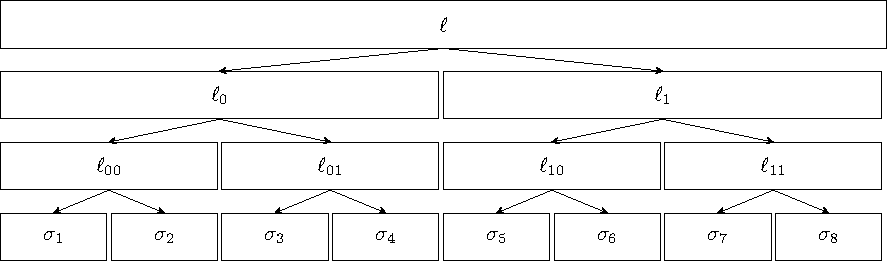
\includegraphics[width=\textwidth]{tikz/FalconTree}
\caption{A \falcon tree of height $3$}\label{fig:falcontree}
\end{figure}

The contents of a \falcon tree \tree are computed from the private key
elements $f$, $g$, $F$ and $G$ using the algorithm described in
\cref{sec:spec:keygen:ffldl} (see also \cref{alg:keygen}).

\subsection{Public key}

The \falcon public key \pk corresponding to the private key $\sk =
(f,g,F,G)$ is a polynomial $h \in \bZ_q[x]/(\phi)$ such that:
 \begin{equation}
  h = gf^{-1} \bmod (\phi,q).
 \end{equation}
